\documentclass[../main.tex]{subfiles}

\begin{document}
    In diesem Abschnitt werden alle Grundlagen der Informatik, die kursübergreifend wichtig sind, zusammengefasst. Dabei geht es vor allem um Begriffsdefinitionen und Konzepte, die in verschiedenen Vorlesungen auftauchen.
    \clearpage

    \section{Informatik}
        Die Definitionen von Informatik unterscheiden sich stark und haben sich im Lauf der Zeit immer weiter an die neuen Erkenntnisse in der Informatik angepasst. Aktuell verwendet die \emph{Gesellschaft für Informatik} diese:
        
        \begin{quote}
            \emph{Wissenschaft, Technik und Anwendung der maschinellen Verarbeitung und Übermittlung von Informationen.}
        \end{quote}
        
    \section{Teilgebiete der Informatik}
        Die Informatik wird in vier Teilgebiete unterteilt.
        
        \paragraph{Theoretische Informatik}
            Die theoretische Informatik beschäftigt sich mit den Konzepten hinter der Informatik auf denen andere Teilgebiete aufbauen und ist aus der Mathematik entstanden. Typische Felder in der theoretischen Informatik sind formale Sprachen, Automatentheorie und die Komplexitäten.
            
        \paragraph{Technische Informatik}
            Die technische Informatik behandelt den Aufbau der Hardware und hat ihre Wurzeln in der Elektortechnik. Typische Felder sind Schaltungstechnologie, Rechnerarchitektur und -organisation sowie Netzwerktechnologie.
            
        \paragraph{Praktische Informatik}
            Die praktische Informatik setzt die Erkenntnisse der theoretischen Informatik unter zuhilfenahme der technischen Informatik mit Algorithmen, Programmiersprachen und der Softwareentwicklung konkret um.
            
        \paragraph{Angewandte Informatik}
            Die angewandte Informatik ist die konkrete Anwendung der praktischen Informatik in der Wirtschaft. Beispiele sind Büroanwendungen wie Textverarbeitung oder Tabellenkalkulation sowie Medizin-Informatik.
        
    \section{Geschichte}
        TODO: An dieser Stelle noch ein paar Worte aus der Geschichte einfügen. Hierfür bieten sich die Folien aus Technische Grundlagen an.
        
    \section{Informationsdarstellung}
        \begin{figure}
             \centering
             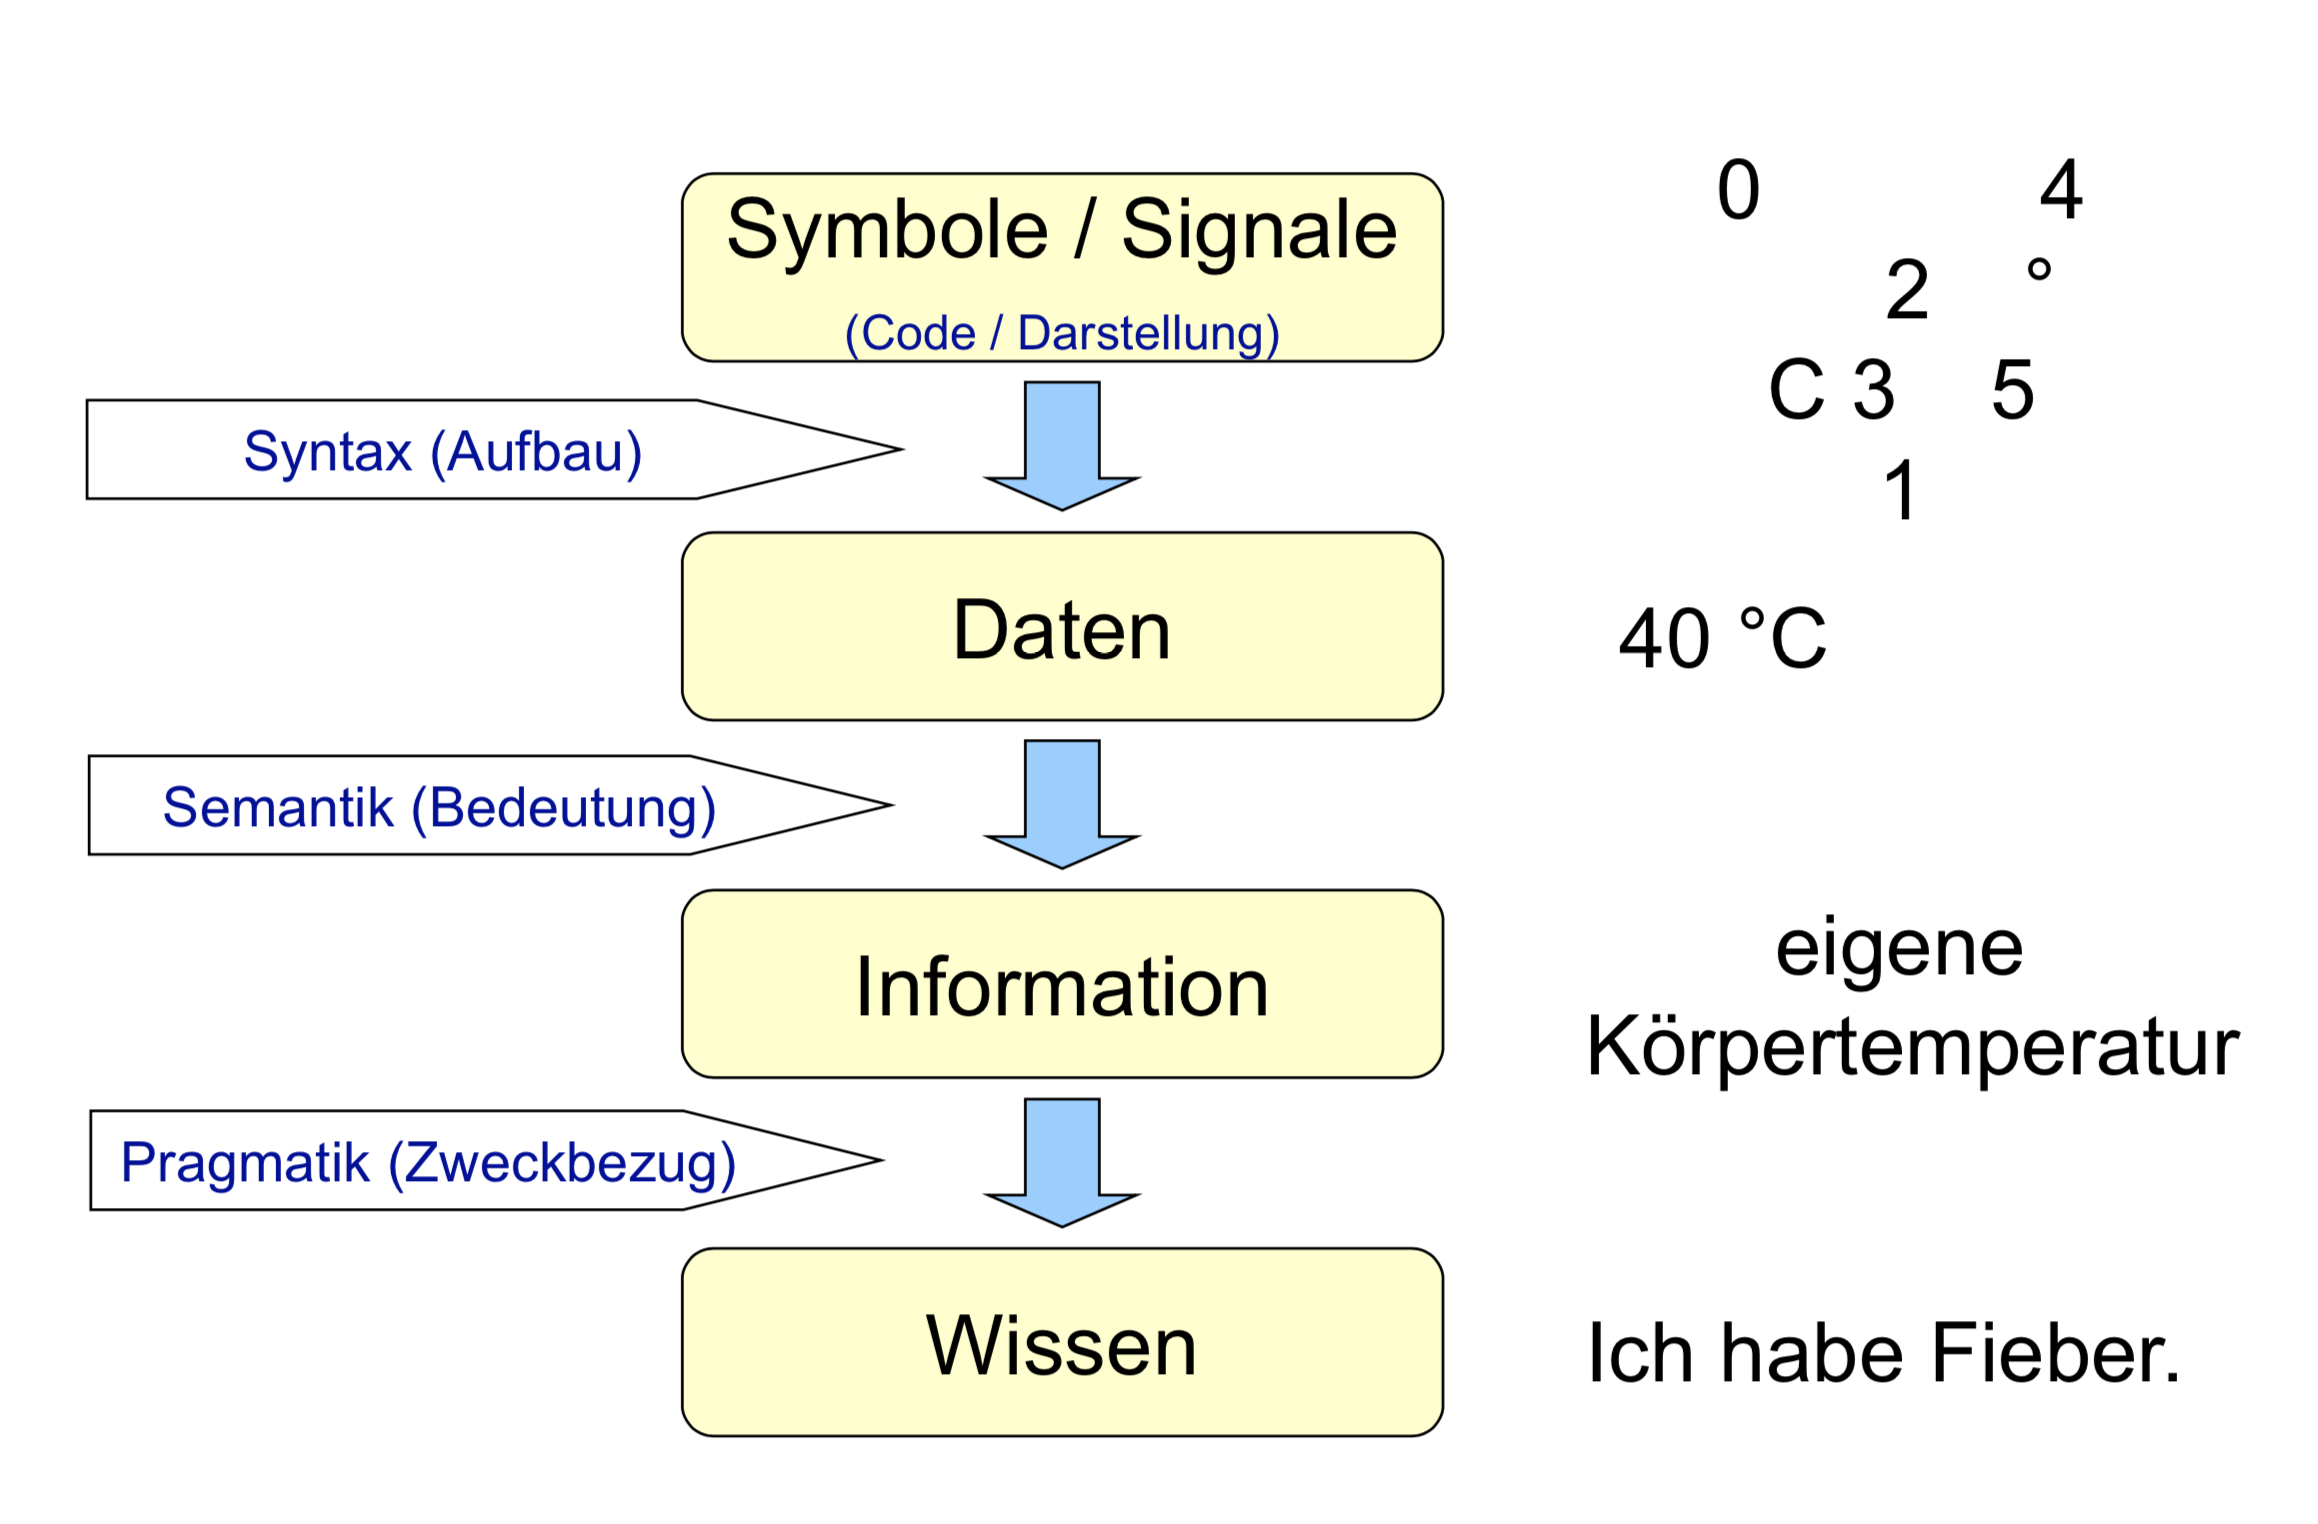
\includegraphics[width=\textwidth]{Abbildungen/Informationsdarstellung.png}
             \caption{Informationsdarstellung}
             \label{figure:Informatik:Grundlagen:informationsdarstellung}
        \end{figure}
    
        Die Informationsdarstellung besteht wie in Abbildung \ref{figure:Informatik:Grundlagen:informationsdarstellung} dargestellt aus verschiedenen Ebenen, die im folgenden weiter erläutert werden.
        
        \paragraph{Signale}
            Signale sind stellen die unterste Ebene dar. Ein Signal ist eine Veränderung einer physikalischen Größe und kann zum Beispiel die Zeichen C$04^\circ$
        
        \paragraph{Daten}
            Um aus Signalen Daten zu machen, muss man eine Syntax anwenden. Ein Beispiel für Daten sind zum Beispiel \SI{40}{\celsius}. Wichtig ist, dass Daten keine Bedeutung haben.
        
        \paragraph{Informationen}
            Informationen sind Teilmengen von Wissen.
            Um von Daten zu Informationen zu kommen, muss man ihnen Eine Semantik zuordnen. Dies ist der Grund dafür, dass Computer nicht in der Lage sind mit Informationen umzugehen. Ein Beispiel für Informationen ist \SI{40}{\celsius} ist die Körpertemperatur.
        
        \paragraph{Wissen}
            Erst mit der Pragmatik kann man aus Informationen Wissen ziehen. Ein Beispiel für Wissen ist, dass es sich um eine erhöhte Temperatur handelt, die auf Fieber hinweist.
        
        \subsection{Darstellbare Informationen}
            Einige Informationen lassen sich als Daten darstellen. Dazu gehöhren unter anderem
        
            \begin{itemize}
                \item Zahlen
                \item Text
                \item logische Werte
                \item Programme
                \item Bilder
                \item Musik
            \end{itemize}
            
            Wie dies umgesetzt wird, wird in \ref{section:Informatik:TechnischeGrundlagen:DarstellungVonInformationen} Darstellung von Informationen thematisiert.
            
    \section{Informationsverarbeitung}
        Da ein Computer nicht in der Lage ist Informationen zu verarbeiten, müssen zunächst immer erst wie in Abbildung \ref{figure:Informatik:Grundlagen:informationsverarbeitung} dargestellt repräsentierende Daten erzeugt werden. Die Daten, die der Computer berechnet müssen anschließend wieder interpretiert werden, um an Informationen zu kommen.
        
        \begin{figure}
             \centering
             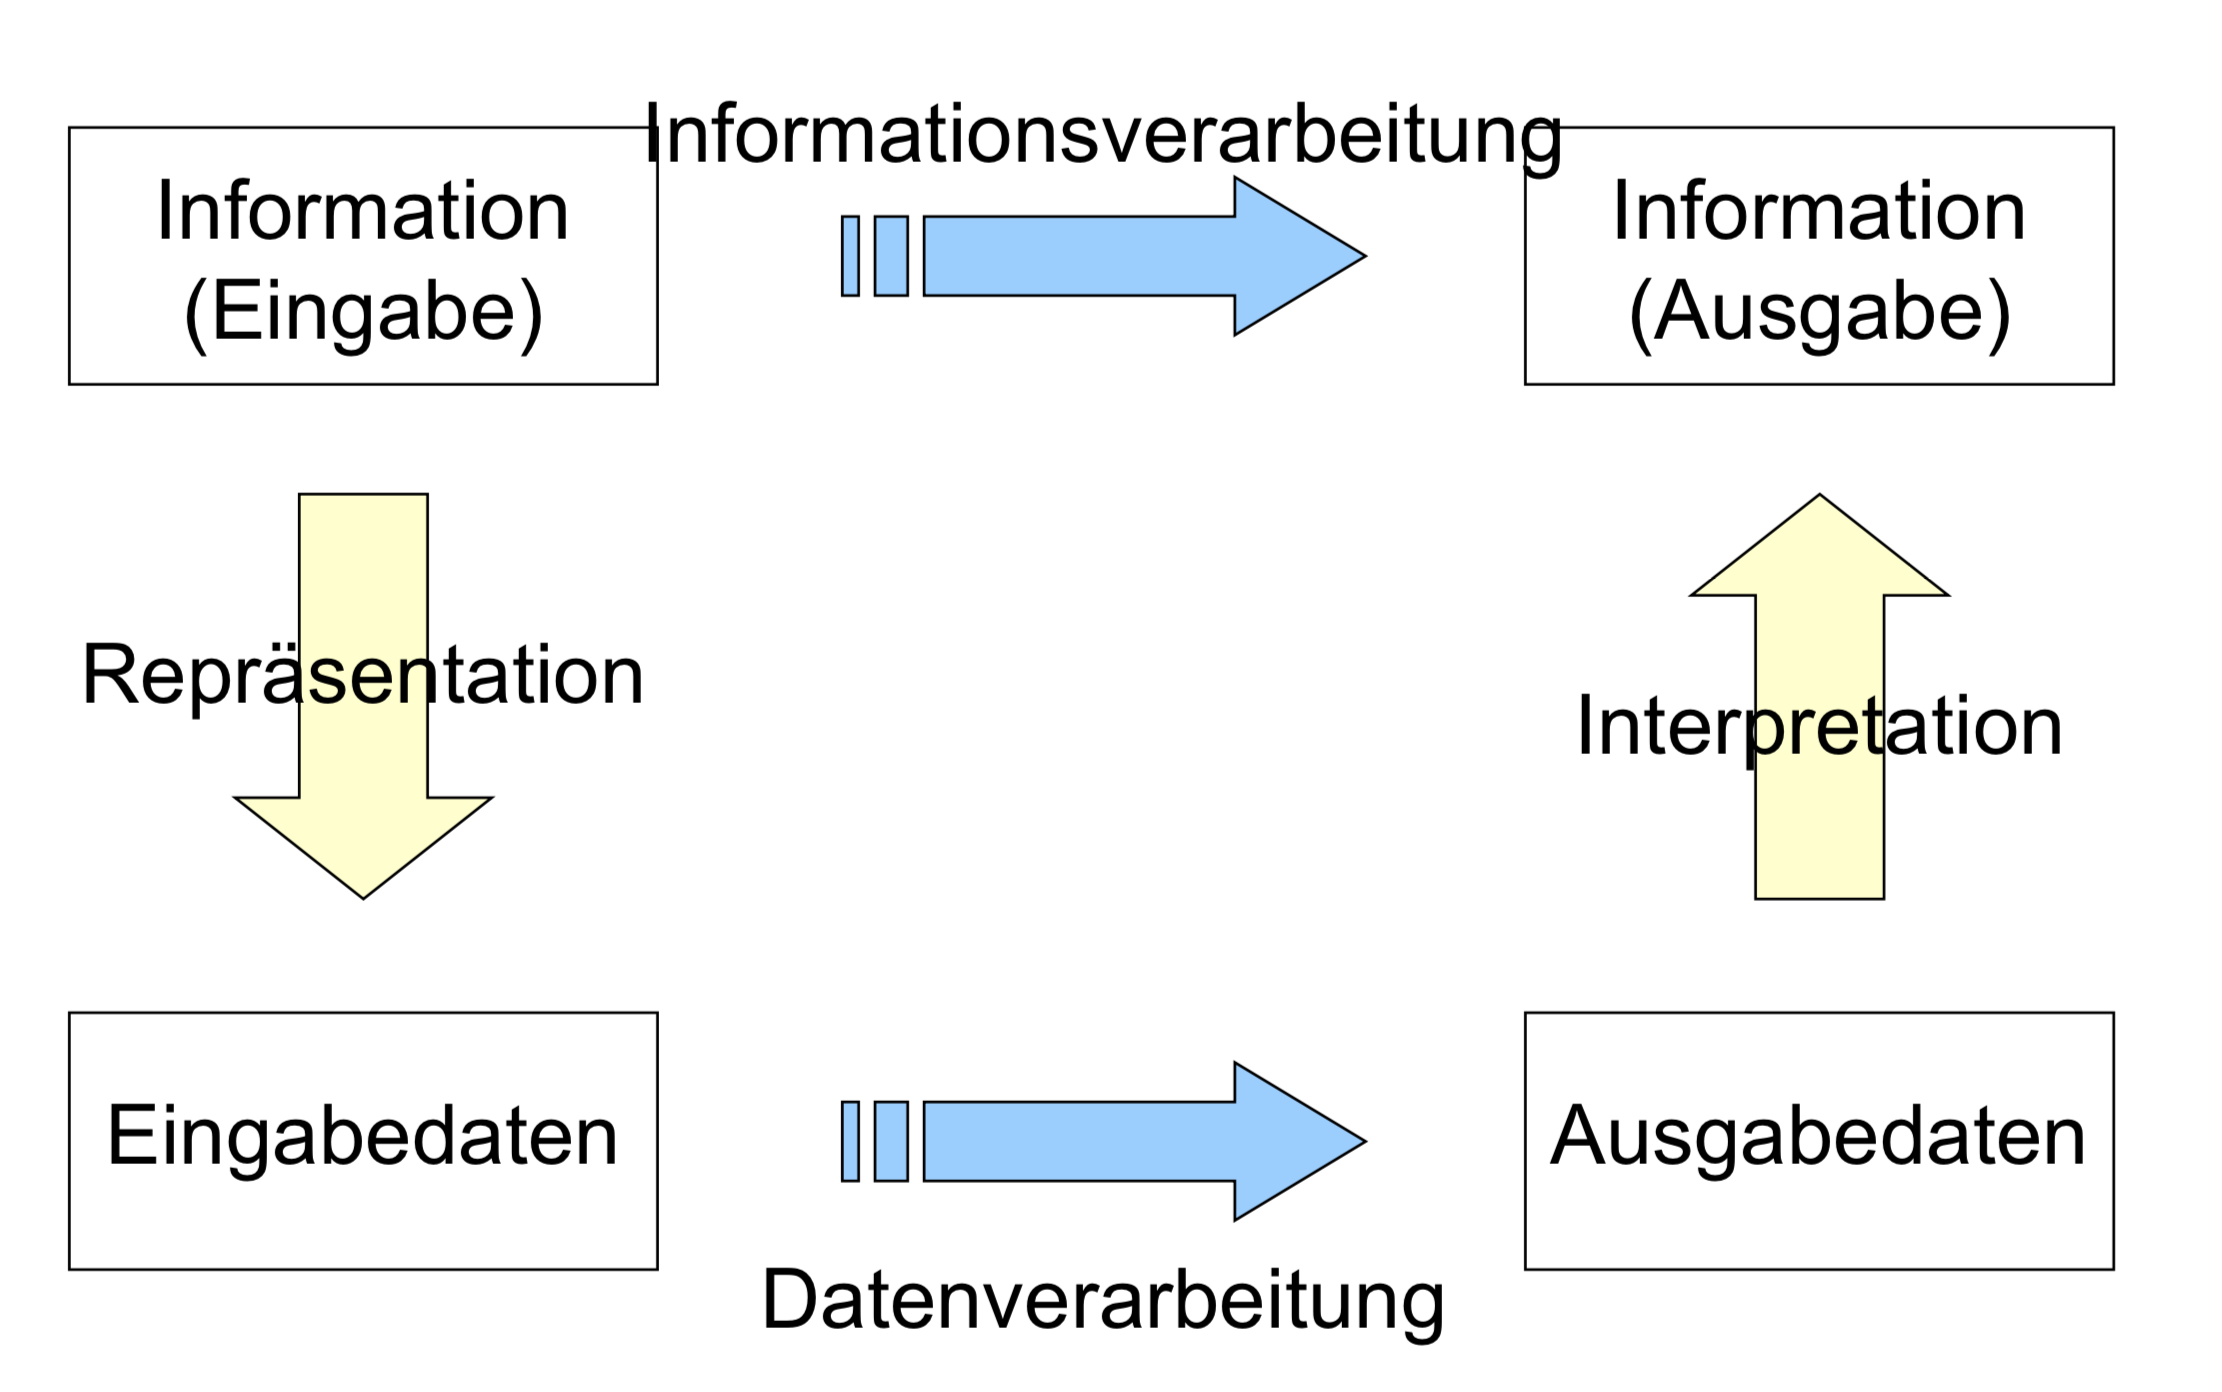
\includegraphics[width=\textwidth]{Abbildungen/Informationsverarbeitung.png}
             \caption{Informationsverarbeitung}
             \label{figure:Informatik:Grundlagen:informationsverarbeitung}
        \end{figure}
    
    \section{Algorithmus}
        Ein Algorithmus ist eine Handlungsvorschrift mit folgenden Eigenschaften:
        
        \begin{itemize}
            \item Der Algorithmus besitzt eine endliche Beschreibung.
            \item Die Beschreibung besteht aus eindeutigen elementaren Anweisungen.
            \item Der nächste Anweisung ist stets deterministisch nur aufgrund von Zwischenergebnissen und der letzten Anweisung festgelegt.
            \item Aus einer endlichen aber belibig großen Eingabe wird eine endliche Ausgabe berechnet.
            \item Es werden endlich viele Schritte benötigt.
        \end{itemize}
    
    \section{Programm}
        Ein Programm ist eine mögliche Implementation eines Algorithmus. Ein Algorithmus kann in verschiedenen Programmiersprachen und verschieden in einer Programmiersprache implementiert werden.
        
    \section{Software}
        Eine Software\footnote{Auch: Software-System, Software-Produkt} ist die Kombination von Programmen, Daten und Dokumentation.
    
    \section{Digitalrechner}
        Ein Digitalrechner\footnote{Digital bedeutet, dass mit diskreten Werten gearbeitet wird. Es bedeutet nicht, dass mit zwei Werten gearbeitet wird.} bedeutet, dass er nicht mit dekreten Ziffern rechnet.
        
    \section{Computer}
        Ein Computer ist ein binärer elektronischer Digitalrechner der
        
        \begin{itemize}
            \item frei programmierbar ist,
            \item einen Arbeitsspeicher zur Daten- und Programmaufnahme besitzt,
            \item die Fähigkeit hat, periphere Ein- und Ausgabegeräte anschließen zu lassen.
        \end{itemize}
        
    \section{Computersystem}
        Ein Computersystem ist die Kombination der Hardware und der Software also ein Computer und Software.
    
\end{document}